

\tikzset{every picture/.style={line width=0.75pt}} %set default line width to 0.75pt        

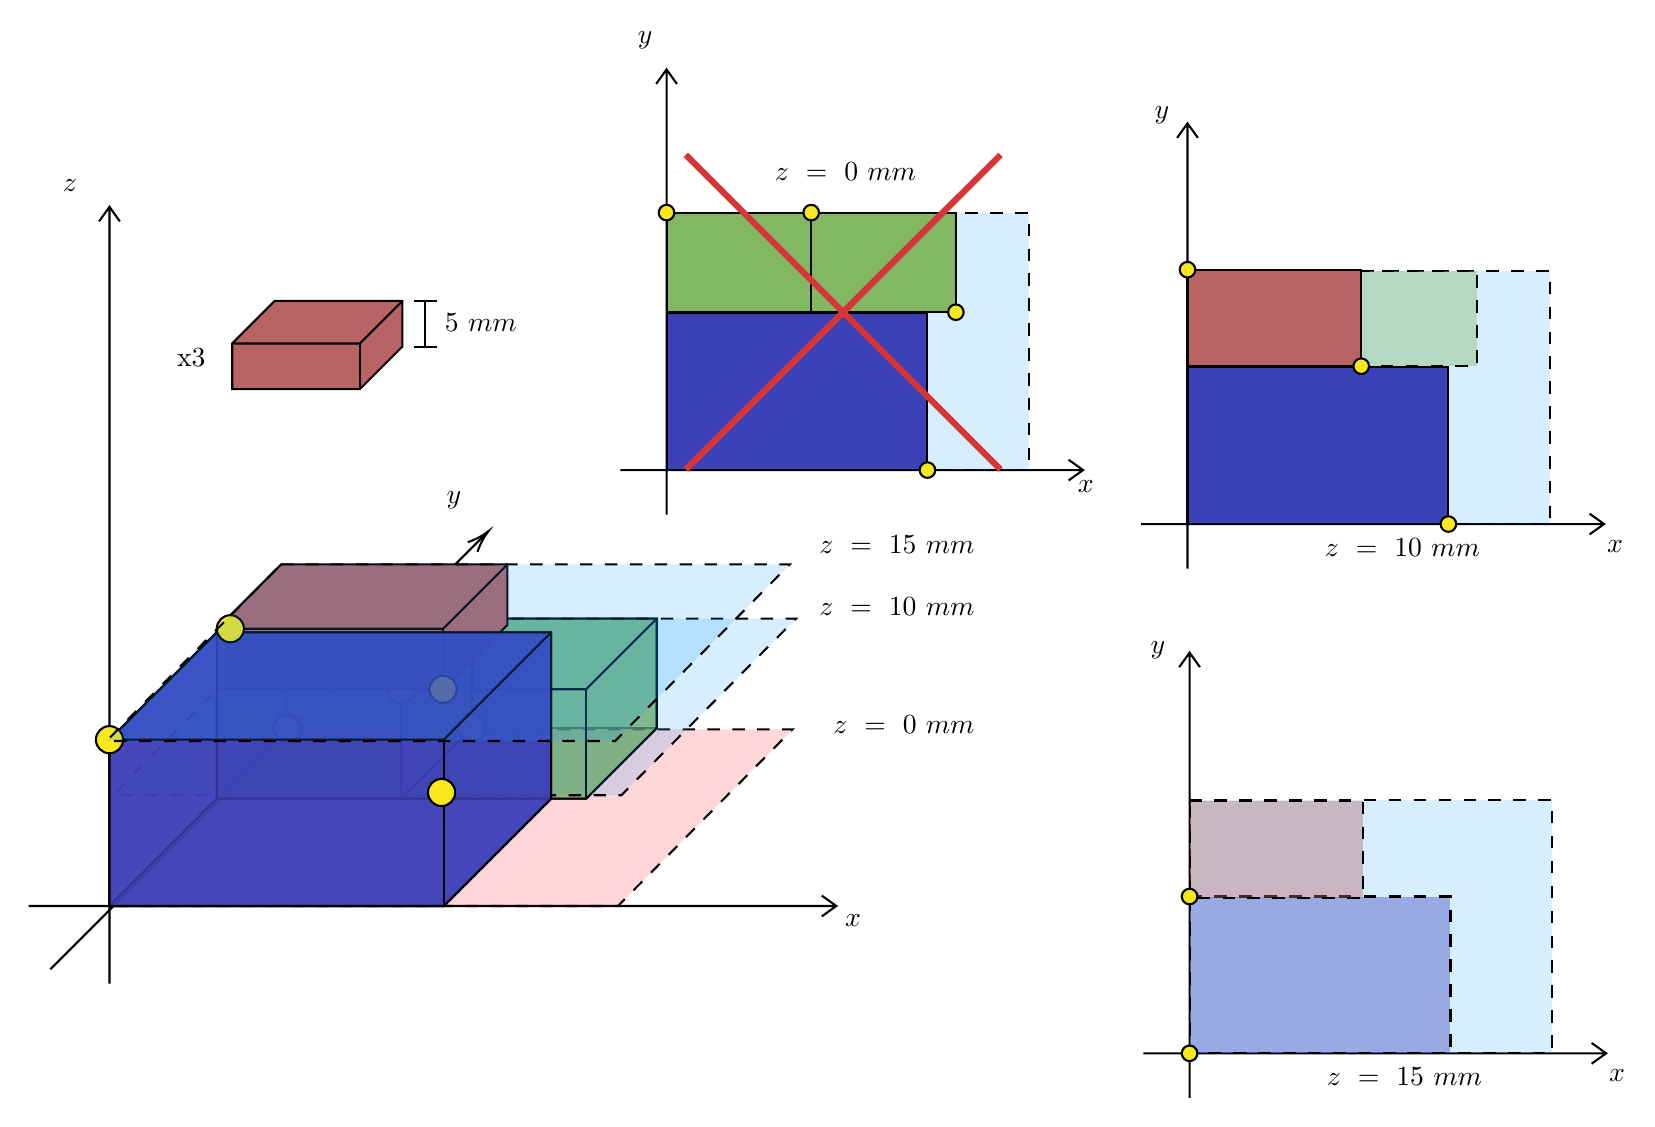
\begin{tikzpicture}[x=0.75pt,y=0.75pt,yscale=-1,xscale=1]
%uncomment if require: \path (0,537); %set diagram left start at 0, and has height of 537

%Shape: Cube [id:dp850859547377836] 
\draw  [fill={rgb, 255:red, 130; green, 184; blue, 100 }  ,fill opacity=0.63 ] (400.59,337.37) -- (366.58,371.38) -- (277.6,371.38) -- (277.6,318.66) -- (311.6,284.65) -- (400.59,284.65) -- cycle ; \draw   (277.6,371.38) -- (311.6,337.37) -- (400.59,337.37) ; \draw   (311.6,337.37) -- (311.6,284.65) ;
%Shape: Parallelogram [id:dp5823195599108398] 
\draw  [fill={rgb, 255:red, 255; green, 17; blue, 34 }  ,fill opacity=0.17 ][dash pattern={on 4.5pt off 4.5pt}] (221,338) -- (466,338) -- (381.91,423.07) -- (136.91,423.07) -- cycle ;
%Shape: Cube [id:dp46134695118901115] 
\draw  [fill={rgb, 255:red, 130; green, 184; blue, 100 }  ,fill opacity=0.63 ] (277.6,318.66) -- (311.6,284.65) -- (400.59,284.65) -- (400.59,337.37) -- (366.58,371.38) -- (277.6,371.38) -- cycle ; \draw   (400.59,284.65) -- (366.58,318.66) -- (277.6,318.66) ; \draw   (366.58,318.66) -- (366.58,371.38) ;
%Shape: Parallelogram [id:dp2915725757037321] 
\draw  [fill={rgb, 255:red, 17; green, 154; blue, 255 }  ,fill opacity=0.17 ][dash pattern={on 4.5pt off 4.5pt}] (222.62,284.65) -- (467.62,284.65) -- (383.53,369.73) -- (138.53,369.73) -- cycle ;
%Shape: Axis 2D [id:dp0385911607889563] 
\draw  (98,423.07) -- (487.11,423.07)(136.91,86.22) -- (136.91,460.5) (480.11,418.07) -- (487.11,423.07) -- (480.11,428.07) (131.91,93.22) -- (136.91,86.22) -- (141.91,93.22)  ;
%Straight Lines [id:da7790786322292883] 
\draw    (108.47,453.52) -- (318.19,243.8) ;
\draw [shift={(319.6,242.39)}, rotate = 135] [color={rgb, 255:red, 0; green, 0; blue, 0 }  ][line width=0.75]    (10.93,-3.29) .. controls (6.95,-1.4) and (3.31,-0.3) .. (0,0) .. controls (3.31,0.3) and (6.95,1.4) .. (10.93,3.29)   ;
%Shape: Cube [id:dp36816769609989985] 
\draw  [fill={rgb, 255:red, 184; green, 100; blue, 100 }  ,fill opacity=1 ] (196.05,152.05) -- (216.55,131.55) -- (278.05,131.55) -- (278.05,153.55) -- (257.55,174.05) -- (196.05,174.05) -- cycle ; \draw   (278.05,131.55) -- (257.55,152.05) -- (196.05,152.05) ; \draw   (257.55,152.05) -- (257.55,174.05) ;
%Straight Lines [id:da34140713541287426] 
\draw    (289.05,131.55) -- (289.05,153.55) ;
\draw [shift={(289.05,153.55)}, rotate = 270] [color={rgb, 255:red, 0; green, 0; blue, 0 }  ][line width=0.75]    (0,5.59) -- (0,-5.59)   ;
\draw [shift={(289.05,131.55)}, rotate = 270] [color={rgb, 255:red, 0; green, 0; blue, 0 }  ][line width=0.75]    (0,5.59) -- (0,-5.59)   ;
%Shape: Cube [id:dp46634170316063617] 
\draw  [fill={rgb, 255:red, 130; green, 184; blue, 100 }  ,fill opacity=0.63 ] (311.6,337.37) -- (277.6,371.38) -- (188.61,371.38) -- (188.61,318.66) -- (222.62,284.65) -- (311.6,284.65) -- cycle ; \draw   (188.61,371.38) -- (222.62,337.37) -- (311.6,337.37) ; \draw   (222.62,337.37) -- (222.62,284.65) ;
%Shape: Cube [id:dp7681025714248981] 
\draw  [fill={rgb, 255:red, 130; green, 184; blue, 100 }  ,fill opacity=0.63 ] (188.61,318.66) -- (222.62,284.65) -- (311.6,284.65) -- (311.6,337.37) -- (277.6,371.38) -- (188.61,371.38) -- cycle ; \draw   (311.6,284.65) -- (277.6,318.66) -- (188.61,318.66) ; \draw   (277.6,318.66) -- (277.6,371.38) ;
%Shape: Ellipse [id:dp06065829561584346] 
\draw  [fill={rgb, 255:red, 248; green, 231; blue, 28 }  ,fill opacity=1 ] (216.07,337.37) .. controls (216.07,333.75) and (219,330.82) .. (222.62,330.82) .. controls (226.23,330.82) and (229.16,333.75) .. (229.16,337.37) .. controls (229.16,340.98) and (226.23,343.91) .. (222.62,343.91) .. controls (219,343.91) and (216.07,340.98) .. (216.07,337.37) -- cycle ;
%Shape: Axis 2D [id:dp6800503914743969] 
\draw  (635,494.05) -- (858,494.05)(657.3,301) -- (657.3,515.5) (851,489.05) -- (858,494.05) -- (851,499.05) (652.3,308) -- (657.3,301) -- (662.3,308)  ;
%Shape: Rectangle [id:dp015242071789025702] 
\draw  [fill={rgb, 255:red, 17; green, 154; blue, 255 }  ,fill opacity=0.17 ][dash pattern={on 4.5pt off 4.5pt}] (657.3,372) -- (832,372) -- (832,494.05) -- (657.3,494.05) -- cycle ;
%Shape: Rectangle [id:dp1874062985177012] 
\draw  [fill={rgb, 255:red, 61; green, 65; blue, 184 }  ,fill opacity=0.4 ][dash pattern={on 4.5pt off 4.5pt}] (657.3,418.5) -- (783,418.5) -- (783,494.05) -- (657.3,494.05) -- cycle ;
%Shape: Circle [id:dp9052763715462506] 
\draw  [fill={rgb, 255:red, 248; green, 231; blue, 28 }  ,fill opacity=1 ] (653.55,494.05) .. controls (653.55,491.98) and (655.23,490.3) .. (657.3,490.3) .. controls (659.37,490.3) and (661.05,491.98) .. (661.05,494.05) .. controls (661.05,496.12) and (659.37,497.8) .. (657.3,497.8) .. controls (655.23,497.8) and (653.55,496.12) .. (653.55,494.05) -- cycle ;
%Shape: Axis 2D [id:dp6870404188341699] 
\draw  (634,239.05) -- (857,239.05)(656.3,46) -- (656.3,260.5) (850,234.05) -- (857,239.05) -- (850,244.05) (651.3,53) -- (656.3,46) -- (661.3,53)  ;
%Shape: Rectangle [id:dp3081187437769213] 
\draw  [fill={rgb, 255:red, 17; green, 154; blue, 255 }  ,fill opacity=0.17 ][dash pattern={on 4.5pt off 4.5pt}] (656.3,117) -- (831,117) -- (831,239.05) -- (656.3,239.05) -- cycle ;
%Shape: Rectangle [id:dp36934590647529786] 
\draw  [fill={rgb, 255:red, 61; green, 65; blue, 184 }  ,fill opacity=1 ] (656.3,163.5) -- (782,163.5) -- (782,239.05) -- (656.3,239.05) -- cycle ;
%Shape: Rectangle [id:dp42040004341602977] 
\draw  [fill={rgb, 255:red, 130; green, 184; blue, 100 }  ,fill opacity=0.4 ][dash pattern={on 4.5pt off 4.5pt}] (656.3,117) -- (726,117) -- (726,163) -- (656.3,163) -- cycle ;
%Shape: Circle [id:dp019789911426076] 
\draw  [fill={rgb, 255:red, 248; green, 231; blue, 28 }  ,fill opacity=1 ] (778.25,239.05) .. controls (778.25,236.98) and (779.93,235.3) .. (782,235.3) .. controls (784.07,235.3) and (785.75,236.98) .. (785.75,239.05) .. controls (785.75,241.12) and (784.07,242.8) .. (782,242.8) .. controls (779.93,242.8) and (778.25,241.12) .. (778.25,239.05) -- cycle ;
%Shape: Rectangle [id:dp7517282497666171] 
\draw  [fill={rgb, 255:red, 130; green, 184; blue, 100 }  ,fill opacity=0.4 ][dash pattern={on 4.5pt off 4.5pt}] (726,117) -- (795.7,117) -- (795.7,163) -- (726,163) -- cycle ;
%Shape: Ellipse [id:dp41816656286565723] 
\draw  [fill={rgb, 255:red, 248; green, 231; blue, 28 }  ,fill opacity=1 ] (305.06,337.37) .. controls (305.06,333.75) and (307.99,330.82) .. (311.6,330.82) .. controls (315.22,330.82) and (318.15,333.75) .. (318.15,337.37) .. controls (318.15,340.98) and (315.22,343.91) .. (311.6,343.91) .. controls (307.99,343.91) and (305.06,340.98) .. (305.06,337.37) -- cycle ;
%Shape: Ellipse [id:dp3000164568050061] 
\draw  [fill={rgb, 255:red, 248; green, 231; blue, 28 }  ,fill opacity=1 ] (271.05,318.66) .. controls (271.05,315.05) and (273.98,312.12) .. (277.6,312.12) .. controls (281.21,312.12) and (284.14,315.05) .. (284.14,318.66) .. controls (284.14,322.28) and (281.21,325.21) .. (277.6,325.21) .. controls (273.98,325.21) and (271.05,322.28) .. (271.05,318.66) -- cycle ;
%Shape: Ellipse [id:dp5080785036195841] 
\draw  [fill={rgb, 255:red, 248; green, 231; blue, 28 }  ,fill opacity=1 ] (290.37,368.37) .. controls (290.37,364.76) and (293.3,361.83) .. (296.91,361.83) .. controls (300.52,361.83) and (303.45,364.76) .. (303.45,368.37) .. controls (303.45,371.98) and (300.52,374.91) .. (296.91,374.91) .. controls (293.3,374.91) and (290.37,371.98) .. (290.37,368.37) -- cycle ;
%Shape: Cube [id:dp7940658414432213] 
\draw  [fill={rgb, 255:red, 184; green, 100; blue, 100 }  ,fill opacity=1 ] (188.61,289.5) -- (219.61,258.5) -- (328.63,258.5) -- (328.63,287.66) -- (297.63,318.66) -- (188.61,318.66) -- cycle ; \draw   (328.63,258.5) -- (297.63,289.5) -- (188.61,289.5) ; \draw   (297.63,289.5) -- (297.63,318.66) ;
%Shape: Cube [id:dp18827267498395128] 
\draw  [fill={rgb, 255:red, 61; green, 65; blue, 184 }  ,fill opacity=0.8 ] (349.7,371.38) -- (298,423.07) -- (136.91,423.07) -- (136.91,342.94) -- (188.61,291.25) -- (349.7,291.25) -- cycle ; \draw   (136.91,423.07) -- (188.61,371.38) -- (349.7,371.38) ; \draw   (188.61,371.38) -- (188.61,291.25) ;
%Shape: Ellipse [id:dp46823065251729934] 
\draw  [fill={rgb, 255:red, 248; green, 231; blue, 28 }  ,fill opacity=1 ] (291.09,318.66) .. controls (291.09,315.05) and (294.02,312.12) .. (297.63,312.12) .. controls (301.24,312.12) and (304.17,315.05) .. (304.17,318.66) .. controls (304.17,322.28) and (301.24,325.21) .. (297.63,325.21) .. controls (294.02,325.21) and (291.09,322.28) .. (291.09,318.66) -- cycle ;
%Shape: Cube [id:dp6823756616236724] 
\draw  [fill={rgb, 255:red, 61; green, 65; blue, 184 }  ,fill opacity=0.8 ] (136.91,342.94) -- (188.61,291.25) -- (349.7,291.25) -- (349.7,371.38) -- (298,423.07) -- (136.91,423.07) -- cycle ; \draw   (349.7,291.25) -- (298,342.94) -- (136.91,342.94) ; \draw   (298,342.94) -- (298,423.07) ;
%Shape: Ellipse [id:dp5738431884006834] 
\draw  [fill={rgb, 255:red, 248; green, 231; blue, 28 }  ,fill opacity=1 ] (130.37,342.94) .. controls (130.37,339.33) and (133.3,336.4) .. (136.91,336.4) .. controls (140.52,336.4) and (143.45,339.33) .. (143.45,342.94) .. controls (143.45,346.56) and (140.52,349.49) .. (136.91,349.49) .. controls (133.3,349.49) and (130.37,346.56) .. (130.37,342.94) -- cycle ;
%Shape: Ellipse [id:dp07646261428683299] 
\draw  [fill={rgb, 255:red, 248; green, 231; blue, 28 }  ,fill opacity=1 ] (188.61,289.5) .. controls (188.61,285.89) and (191.54,282.96) .. (195.15,282.96) .. controls (198.77,282.96) and (201.69,285.89) .. (201.69,289.5) .. controls (201.69,293.11) and (198.77,296.04) .. (195.15,296.04) .. controls (191.54,296.04) and (188.61,293.11) .. (188.61,289.5) -- cycle ;
%Shape: Parallelogram [id:dp08950497007303859] 
\draw  [fill={rgb, 255:red, 17; green, 154; blue, 255 }  ,fill opacity=0.17 ][dash pattern={on 4.5pt off 4.5pt}] (219.61,258.5) -- (464.61,258.5) -- (380.52,343.57) -- (135.52,343.57) -- cycle ;
%Shape: Rectangle [id:dp4478205527448239] 
\draw  [fill={rgb, 255:red, 184; green, 100; blue, 100 }  ,fill opacity=1 ] (656.3,116.5) -- (740,116.5) -- (740,163) -- (656.3,163) -- cycle ;
%Shape: Circle [id:dp13454299239933898] 
\draw  [fill={rgb, 255:red, 248; green, 231; blue, 28 }  ,fill opacity=1 ] (736.25,163) .. controls (736.25,160.93) and (737.93,159.25) .. (740,159.25) .. controls (742.07,159.25) and (743.75,160.93) .. (743.75,163) .. controls (743.75,165.07) and (742.07,166.75) .. (740,166.75) .. controls (737.93,166.75) and (736.25,165.07) .. (736.25,163) -- cycle ;
%Shape: Circle [id:dp8773584456012923] 
\draw  [fill={rgb, 255:red, 248; green, 231; blue, 28 }  ,fill opacity=1 ] (652.55,116.5) .. controls (652.55,114.43) and (654.23,112.75) .. (656.3,112.75) .. controls (658.37,112.75) and (660.05,114.43) .. (660.05,116.5) .. controls (660.05,118.57) and (658.37,120.25) .. (656.3,120.25) .. controls (654.23,120.25) and (652.55,118.57) .. (652.55,116.5) -- cycle ;
%Shape: Rectangle [id:dp6527670874867769] 
\draw  [fill={rgb, 255:red, 184; green, 100; blue, 100 }  ,fill opacity=0.4 ][dash pattern={on 4.5pt off 4.5pt}] (657.3,372.5) -- (741,372.5) -- (741,419) -- (657.3,419) -- cycle ;
%Shape: Circle [id:dp2657813756631938] 
\draw  [fill={rgb, 255:red, 248; green, 231; blue, 28 }  ,fill opacity=1 ] (653.55,418.5) .. controls (653.55,416.43) and (655.23,414.75) .. (657.3,414.75) .. controls (659.37,414.75) and (661.05,416.43) .. (661.05,418.5) .. controls (661.05,420.57) and (659.37,422.25) .. (657.3,422.25) .. controls (655.23,422.25) and (653.55,420.57) .. (653.55,418.5) -- cycle ;
%Shape: Ellipse [id:dp22740515272810635] 
\draw  [fill={rgb, 255:red, 248; green, 231; blue, 28 }  ,fill opacity=1 ] (290.37,368.37) .. controls (290.37,364.76) and (293.3,361.83) .. (296.91,361.83) .. controls (300.52,361.83) and (303.45,364.76) .. (303.45,368.37) .. controls (303.45,371.98) and (300.52,374.91) .. (296.91,374.91) .. controls (293.3,374.91) and (290.37,371.98) .. (290.37,368.37) -- cycle ;
%Shape: Axis 2D [id:dp28534705658973836] 
\draw  (383,213.05) -- (606,213.05)(405.3,20) -- (405.3,234.5) (599,208.05) -- (606,213.05) -- (599,218.05) (400.3,27) -- (405.3,20) -- (410.3,27)  ;
%Shape: Rectangle [id:dp34444980481385135] 
\draw  [fill={rgb, 255:red, 17; green, 154; blue, 255 }  ,fill opacity=0.17 ][dash pattern={on 4.5pt off 4.5pt}] (405.3,89) -- (580,89) -- (580,213.05) -- (405.3,213.05) -- cycle ;
%Shape: Rectangle [id:dp6600565254726414] 
\draw  [fill={rgb, 255:red, 61; green, 65; blue, 184 }  ,fill opacity=1 ] (405.3,137.5) -- (531,137.5) -- (531,213.05) -- (405.3,213.05) -- cycle ;
%Shape: Circle [id:dp687328768761151] 
\draw  [fill={rgb, 255:red, 248; green, 231; blue, 28 }  ,fill opacity=1 ] (527.25,213.05) .. controls (527.25,210.98) and (528.93,209.3) .. (531,209.3) .. controls (533.07,209.3) and (534.75,210.98) .. (534.75,213.05) .. controls (534.75,215.12) and (533.07,216.8) .. (531,216.8) .. controls (528.93,216.8) and (527.25,215.12) .. (527.25,213.05) -- cycle ;
%Shape: Rectangle [id:dp4720998169870536] 
\draw  [fill={rgb, 255:red, 130; green, 184; blue, 100 }  ,fill opacity=1 ] (405.3,89) -- (475,89) -- (475,137) -- (405.3,137) -- cycle ;
%Shape: Circle [id:dp2451407265899025] 
\draw  [fill={rgb, 255:red, 248; green, 231; blue, 28 }  ,fill opacity=1 ] (401.55,89) .. controls (401.55,86.93) and (403.23,85.25) .. (405.3,85.25) .. controls (407.37,85.25) and (409.05,86.93) .. (409.05,89) .. controls (409.05,91.07) and (407.37,92.75) .. (405.3,92.75) .. controls (403.23,92.75) and (401.55,91.07) .. (401.55,89) -- cycle ;
%Shape: Rectangle [id:dp9804240171062975] 
\draw  [fill={rgb, 255:red, 130; green, 184; blue, 100 }  ,fill opacity=1 ] (475,89) -- (544.7,89) -- (544.7,137) -- (475,137) -- cycle ;
%Shape: Circle [id:dp3092275472196101] 
\draw  [fill={rgb, 255:red, 248; green, 231; blue, 28 }  ,fill opacity=1 ] (540.95,137) .. controls (540.95,134.93) and (542.63,133.25) .. (544.7,133.25) .. controls (546.77,133.25) and (548.45,134.93) .. (548.45,137) .. controls (548.45,139.07) and (546.77,140.75) .. (544.7,140.75) .. controls (542.63,140.75) and (540.95,139.07) .. (540.95,137) -- cycle ;
%Shape: Circle [id:dp07506811257370083] 
\draw  [fill={rgb, 255:red, 248; green, 231; blue, 28 }  ,fill opacity=1 ] (471.25,89) .. controls (471.25,86.93) and (472.93,85.25) .. (475,85.25) .. controls (477.07,85.25) and (478.75,86.93) .. (478.75,89) .. controls (478.75,91.07) and (477.07,92.75) .. (475,92.75) .. controls (472.93,92.75) and (471.25,91.07) .. (471.25,89) -- cycle ;
\draw  [color={rgb, 255:red, 214; green, 54; blue, 54 }  ,draw opacity=1 ][line width=2.25]  (414.59,61.2) -- (566.2,212.8)(566.2,61.2) -- (414.59,212.8) ;

% Text Node
\draw (484.19,329.66) node [anchor=north west][inner sep=0.75pt]    {$z\ =\ 0\ mm$};
% Text Node
\draw (297.9,221.7) node [anchor=north west][inner sep=0.75pt]    {$y$};
% Text Node
\draw (489.84,425.85) node [anchor=north west][inner sep=0.75pt]    {$x$};
% Text Node
\draw (112.94,71.64) node [anchor=north west][inner sep=0.75pt]    {$z$};
% Text Node
\draw (168,153) node [anchor=north west][inner sep=0.75pt]   [align=left] {x3};
% Text Node
\draw (297.05,135.95) node [anchor=north west][inner sep=0.75pt]    {$5\ mm$};
% Text Node
\draw (477.48,243.2) node [anchor=north west][inner sep=0.75pt]    {$z\ =\ 15\ mm$};
% Text Node
\draw (858,500.4) node [anchor=north west][inner sep=0.75pt]    {$x$};
% Text Node
\draw (639,36.4) node [anchor=north west][inner sep=0.75pt]    {$y$};
% Text Node
\draw (722,499.4) node [anchor=north west][inner sep=0.75pt]    {$z\ =\ 15\ mm$};
% Text Node
\draw (477.48,273.2) node [anchor=north west][inner sep=0.75pt]    {$z\ =\ 10\ mm$};
% Text Node
\draw (857,245.4) node [anchor=north west][inner sep=0.75pt]    {$x$};
% Text Node
\draw (721,244.4) node [anchor=north west][inner sep=0.75pt]    {$z\ =\ 10\ mm$};
% Text Node
\draw (390,0.4) node [anchor=north west][inner sep=0.75pt]    {$y$};
% Text Node
\draw (456,63.4) node [anchor=north west][inner sep=0.75pt]    {$z\ =\ 0\ mm$};
% Text Node
\draw (637,294.4) node [anchor=north west][inner sep=0.75pt]    {$y$};
% Text Node
\draw (602,216.4) node [anchor=north west][inner sep=0.75pt]    {$x$};


\end{tikzpicture}
